\documentclass[a4paper]{article}
\usepackage{amsmath}
\usepackage{multicol} % Multiple columns
\usepackage{graphicx} % Image including
\usepackage{float} % Floats positioning (allows fixed)
\usepackage[landscape,a4paper,twoside=false,top=15mm,bottom=15mm,left=10mm,right=10mm]{geometry} % Document margins
\pagestyle{myheadings}
\markright{}
\usepackage{listings}
\usepackage{color}
\usepackage{hyperref}
\lstset{ % Configure 
    tabsize=4,
    basicstyle=\ttfamily\scriptsize,
    aboveskip={0\baselineskip},
    columns=fixed,
    showstringspaces=false,
    extendedchars=true,
    breaklines=true,
    prebreak = \raisebox{0ex}[0ex][0ex]{\ensuremath{\hookleftarrow}},
    frame=single,
    rulecolor=\color[rgb]{0.75,0.75,0.75},
    showtabs=false,
    showspaces=false,
    showstringspaces=false,
    keywordstyle=\color[rgb]{0,0,1},
    commentstyle=\color[rgb]{0.133,0.545,0.133},
    stringstyle=\color[rgb]{0.627,0.126,0.941},
    numbers=left,
    numberstyle=\tiny,
    numbersep=7pt,
    xleftmargin=0.5cm,
}
\lstset{emph={% Add keywords from C++ and Template
    vll,ll,ld,pll,vpll,F,FF,REP,FOR,pb,dbg,EPS,INF,CL,all,size,IN,string,pair,map,set,unordered_map,vector,unordered_set,queue,priority_queue,list%
    },emphstyle={\color{blue}}%
}
\widowpenalty=10000 % Breaking before last line of a paragraph
\clubpenalty=10000 % Breaking after first line of paragraph
\setlength{\parindent}{0.0in}

\begin{document}
\begin{multicols*}{2}
\setlength{\parskip}{0.0in}
\tableofcontents
\setlength{\parskip}{0.1in}

\section{Strings}
    \subsection{Knuth - Morris - Pratt algorithm}
        \lstinputlisting[language=c++,firstline=3]{../strings/kmp.cpp}
    \subsection{Manacher's longest pallindromic substring}
        \lstinputlisting[language=c++,firstline=3]{../strings/manacher.cpp}
    \subsection{Aho-Corasick}
        \lstinputlisting[language=c++,firstline=3]{../strings/aho.cpp}
    \subsection{Rabin-Karp (Rolling hash)}
        \lstinputlisting[language=c++,firstline=3]{../strings/rabin-karp.cpp}
    \subsection{Boyer-moore}
        \lstinputlisting[language=c++,firstline=3,lastline=50]{../strings/boyer-moore.cpp}
    \subsection{Suffix array + Longest common prefix}
        \lstinputlisting[language=c++,firstline=3]{../strings/suffixArray+LCE.cpp}

\section{Graphs}
    \subsection{DFS/BFS like}
        \subsubsection{DFS and BFS}
            \lstinputlisting[language=c++]{../graphs/dbfs.cpp}
        \subsubsection{Toposort (using DFS)}
            \lstinputlisting[language=c++]{../graphs/topoDFS.cpp}
        \subsubsection{Toposort (using list cutting)}
            \lstinputlisting[language=c++]{../graphs/topoListCut.cpp}
        \subsubsection{Bipartity check}
            \lstinputlisting[language=c++]{../graphs/bipartite.cpp}
        \subsubsection{Articulations \& bridges}
            \lstinputlisting[language=c++]{../graphs/articulations-bridges.cpp}

    \subsection{Shortest path}
        \subsubsection{Dijkstra's algorithm}
            \lstinputlisting[language=c++]{../graphs/dijkstra.cpp}
        \subsubsection{Bellman Ford's algorithm}
            \lstinputlisting[language=c++]{../graphs/bellford.cpp}
        \subsubsection{Floyd--Warshall's algorithm}
            \lstinputlisting[language=c++,firstline=3]{../graphs/fw.cpp}
        \subsubsection{Johnson's algorithm}
            \lstinputlisting[language=c++]{../graphs/bellford.cpp}
    
    \subsection{Flows (Ford Fulkersons)}
        \subsubsection{Edmonds--Karp's algorithm}
            \lstinputlisting[language=c++]{../graphs/edmondKarp.cpp}
        \subsubsection{Dinic's algorithm}
            \lstinputlisting[language=c++,firstline=3]{../graphs/dinic.cpp}
        \subsubsection{Hopcroft–Karp bipartite maximal matching (BFS)}
            \lstinputlisting[language=c++]{../graphs/hopcroftKarp.cpp}
        \subsubsection{Bipartite maximal matching (DFS)}
            \lstinputlisting[language=c++]{../graphs/bipartite_matching.cpp}

    \subsection{Spanning trees}
        \subsubsection{Kruskal-Boruvka}
            \lstinputlisting[language=c++]{../graphs/kruskal.cpp}
        \subsubsection{Jarnik-Prim}
            \lstinputlisting[language=c++]{../graphs/jarnik.cpp}
    \subsection{Hard problems}
        \subsubsection{Travelling salesman problem -- TSP}
            \lstinputlisting[language=c++]{../graphs/tsp.cpp}
        \subsubsection{Hamiltonian path}
            \lstinputlisting[language=c++]{../graphs/hamiltonian_path.cpp}
        \subsubsection{Eulerian path}
            \lstinputlisting[language=c++]{../graphs/euler.cpp}
        \subsubsection{Vertex cover}
            \lstinputlisting[language=c++]{../graphs/vertexCover.cpp}

\section{Data structures}
    \subsection{Union find}
        \lstinputlisting[language=c++]{../structs/union_find.cpp}
    \subsection{Fenwick tree}
        \lstinputlisting[language=c++]{../structs/fenwick_tree.cpp}
    \subsection{Segment tree}
        \lstinputlisting[language=c++]{../structs/segmentTree.cpp}
    \subsection{Segment tree Lazy}
        \lstinputlisting[language=c++]{../structs/segmentTreeLazy.cpp}
    \subsection{Range Minimum Query (RMQ)}
        \lstinputlisting[language=c++]{../structs/rmq.cpp}
    \subsection{Lowest Common Ancestor (LCA)}
        \lstinputlisting[language=c++]{../structs/lca.cpp}
    \subsection{LCA iterative}
        \lstinputlisting[language=c++]{../structs/lca2.cpp}
    \subsection{Tarjan's offline LCA}
        \lstinputlisting[language=c++]{../structs/lca3.cpp}
    \subsection{Treap}
        \lstinputlisting[language=c++]{../structs/treap.cpp}
    \subsection{Key Order Set}
        \lstinputlisting[language=c++]{../structs/keyOrderSet.cpp}
    \subsection{Key-Value structure with access by key and getMax operation}
        \lstinputlisting[language=c++]{../structs/arrayWithGetMax.cpp}
    \subsection{HLD}
        \lstinputlisting[language=c++]{../structs/hld.cpp}
    \subsection{HLD2}
            \lstinputlisting[language=c++]{../structs/hl2.cpp}

\section{Math}
    \subsection{List divisors}
        \lstinputlisting[language=c++]{../math/divisors.cpp}
    \subsection{Modular inverse}
        \lstinputlisting[language=c++]{../math/mod_inverse.cpp}
    \subsection{Prime and Factorization sieve in O(n)}
        \lstinputlisting[language=c++,firstline=3]{../math/eraLinear.cpp}
    \subsection{Sieve of Eratosthenes}
        \lstinputlisting[language=c++]{../math/era.cpp}
    \subsection{Euclidean algorithm}
        \subsubsection{Euclidean algorithm (GCD)}
            \lstinputlisting[language=c++]{../math/gcd.cpp}
        \subsubsection{Extended Euclidean algorithm (EGCD)}
            \lstinputlisting[language=c++]{../math/extended_euclid.cpp}
    \subsection{Pascal's triangle}
        \lstinputlisting[language=c++]{../math/pascal.cpp}
    \subsection{Powers}
        \subsubsection{Power of number}
            \lstinputlisting[language=c++]{../math/power.cpp}
        \subsubsection{Modular power}
            \lstinputlisting[language=c++]{../math/powmod.cpp}
        \subsubsection{Matrix power}
            \lstinputlisting[language=c++]{../math/matrix_exponentiation.cpp}
    \subsection{Equations}
        \subsubsection{Gauss elimination method -- GEM}
            \lstinputlisting[language=c++]{../math/gem.cpp}
        \subsubsection{Linear diophantine (ax+by=c)}
            \lstinputlisting[language=c++]{../math/linear_diophantine.cpp}
        \subsubsection{Modular linear equation (ax=b mod m)}
            \lstinputlisting[language=c++]{../math/modular_linear_equation_solver.cpp}
        \subsubsection{Recurrent equations}
            \lstinputlisting[language=c++]{../math/recurrent.cpp}
        \subsubsection{Recurrent equations 2}
            \lstinputlisting[language=c++]{../math/recurrent2.cpp}
    \subsection{Factorization}
        \lstinputlisting[language=c++]{../math/factorization.cpp }
    \subsection{Rabin Miller test}
        \lstinputlisting[language=c++]{../math/rabin-miller.cpp}
    \subsection{Chinese reminder theorem}
        \lstinputlisting[language=c++]{../math/chinese.cpp}
    \subsection{Big numbers in Java}
        \lstinputlisting[language=java]{../math/bignumJava.java}
    \subsection{Big numbers}
        \lstinputlisting[language=c++]{../math/bignum.cpp}
    \subsection{Catalan numbers}
        \lstinputlisting[language=c++]{../math/catalan.cpp}
    \subsection{Combinatinal numbers}
        \lstinputlisting[language=c++]{../math/comb.cpp}
    \subsection{Combinatinal numbers modulo}
        \lstinputlisting[language=c]{../math/comb_mod.c}
    \subsection{Euler's totient function}
        \lstinputlisting[language=c]{../math/eulersTotientFunc.cpp}
    \subsection{Fast polynom multiplication using DFFT}
        \lstinputlisting[language=c]{../math/fft.cpp}
    \subsection{Horner's rule for evaluation of polynoms}
        \lstinputlisting[language=c]{../math/horner.cpp}

\section{Geometry}
    \subsection{Global features}
        \lstinputlisting[language=c++]{../geometry/geometry.cpp}
    \subsection{Line equation}
        \lstinputlisting[language=c++]{../geometry/line_equation.cpp }
    \subsection{Circles}
        \subsubsection{Circle-line intersection}
            \lstinputlisting[language=c++]{../geometry/circleLineInters.cpp}
        \subsubsection{Two circles intersection}
            \lstinputlisting[language=c++]{../geometry/2circlesInters.cpp}
        \subsubsection{Triangles: inscribed + circumscribed circle}
            \lstinputlisting[language=c++]{../geometry/circle-inscribed-circumscribed.cpp}
        \subsubsection{Triangles \& quadrilaterals facts}
            \lstinputlisting[language=c++]{../geometry/triangles-quadrilaterals.cpp}
        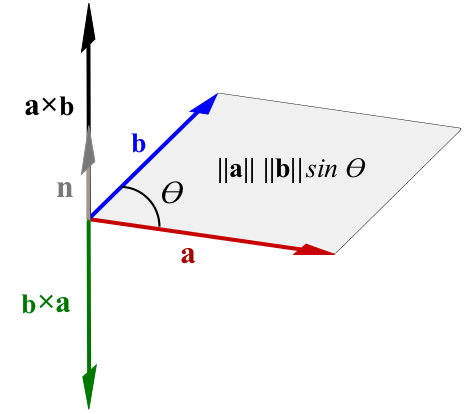
\includegraphics[width=6.5cm]{../images/Cross-product-with-area.png}
        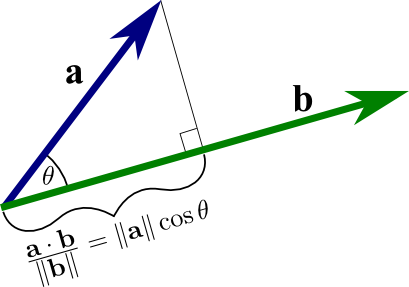
\includegraphics[width=6.5cm]{../images/dot_product_projection.png}
    \subsection{Convex hull}
        \lstinputlisting[language=c++]{../geometry/convex_hull.cpp}
    \subsection{3D geometry}
        \subsubsection{Gloabal features}
            \lstinputlisting[language=c++]{../geometry/3dgeometry.cpp}
        \subsubsection{Spherical distance}
            \lstinputlisting[language=c++]{../geometry/3d-spherical-distance.cpp}

\section{Dynamic programming}
    \subsection{Longest increasing subsequence}
        \lstinputlisting[language=c++]{../dp/lis.cpp}
    \subsection{Minimal cost path}
        \lstinputlisting[language=c++]{../dp/minCostPath.cpp}

\section{Others}
    \subsection{Binary search}
        \lstinputlisting[language=c++]{../other/binary.cpp}
    \subsection{Ternary search}
        \lstinputlisting[language=c++]{../other/ternary_search.c}
    \subsection{Bit tricks}
        \lstinputlisting[language=c++]{../other/miscellaneous.cpp}
    \subsection{Gray code}
        \lstinputlisting[language=c++]{../other/grayCode.cpp}
    \subsection{K-th minimum}
        \lstinputlisting[language=c++]{../other/kthMin.cpp}
    \subsection{All nearest smaller values}
        \lstinputlisting[language=c++]{../other/allNearestSmaller.cpp}
    \subsection{STL}
        \lstinputlisting[language=c++]{../other/stl.cpp}
    \subsection{Template}
        \lstinputlisting[language=c++]{../template.cpp}
    \subsection{.bash-profile}
        \lstinputlisting[language=bash]{../other/basrc}
    \subsection{.vimrc}
        \lstinputlisting[language=bash]{../other/vimrc}
    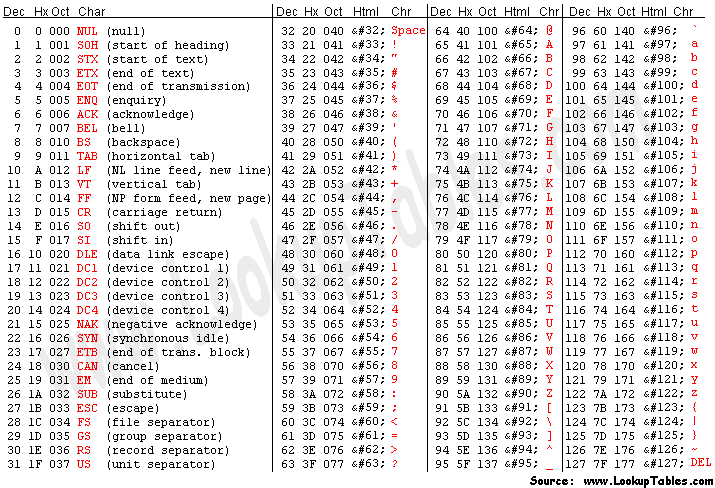
\includegraphics[width=\linewidth]{../other/asciifull.png}

\end{multicols*}
\end{document}